\documentclass[12pt]{report}
\usepackage{graphicx} % Required for inserting images
\usepackage{multirow}
\usepackage{lscape}
\usepackage{pdflscape}
\usepackage{fixltx2e}
\usepackage{geometry}
\usepackage{wasysym}
\usepackage{amsmath}
\usepackage{amssymb}
\usepackage{caption}
\usepackage{subcaption}


\newcommand{\head}[1]{\textnormal{\textbf{#1}}}
\newcommand\ion[2]{\text{#1\,\textsc{\lowercase{#2}}}}

\title{\textbf{System plots}}
% \date{}

\begin{document}

\maketitle




\begin{landscape}

    \begin{figure}
    \centering
    \vspace{-20mm}
    \hspace*{-35mm}
    \captionsetup{oneside,margin={0cm,35mm}}
    \includegraphics[width=1.25\linewidth]{sys_plots_full/3C263_z=0.140756_sys_plot_full.png}
    \end{figure}
    
\end{landscape}

\textbf{Comments:}

\begin{itemize}
    \item $\Delta v = [-100,100]$
\end{itemize}



\begin{landscape}

    \begin{figure}
    \centering
    \vspace{-20mm}
    \hspace*{-35mm}
    \captionsetup{oneside,margin={0cm,35mm}}
    \includegraphics[width=1.25\linewidth]{sys_plots_full/PKS0637-752_z=0.161064_sys_plot_full.png}
    \end{figure}
    
\end{landscape}

\textbf{Comments:}

\begin{itemize}
    \item $\Delta v = [-100,100]$
    \item \ion{Fe}{ii} 1144 : contaminated with \ion{H}{i} 937 from z=0.417415
\end{itemize}


\begin{landscape}

    \begin{figure}
    \centering
    \vspace{-20mm}
    \hspace*{-35mm}
    \captionsetup{oneside,margin={0cm,35mm}}
    \includegraphics[width=1.25\linewidth]{sys_plots_full/PKS0637-752_z=0.417539_sys_plot_full.png}
    \end{figure}
    
\end{landscape}

\textbf{Comments:}

\begin{itemize}
    \item $\Delta v = [-100,100]$
    \item \ion{O}{iii} 832 : contaminated with galactic \ion{Si}{iv} 1402
\end{itemize}


\begin{landscape}

    \begin{figure}
    \centering
    \vspace{-20mm}
    \hspace*{-35mm}
    \captionsetup{oneside,margin={0cm,35mm}}
    \includegraphics[width=1.25\linewidth]{sys_plots_full/PG1424+240_z=0.147104_sys_plot_full.png}
    \end{figure}
    
\end{landscape}


\textbf{Comments:}

\begin{itemize}
    \item $\Delta v = [-130,80]$
    \item \ion{C}{ii} 1036 : contaminated with galactic \ion{C}{i} 1188
\end{itemize}


\begin{landscape}

    \begin{figure}
    \centering
    \vspace{-20mm}
    \hspace*{-35mm}
    \captionsetup{oneside,margin={0cm,35mm}}
    \includegraphics[width=1.25\linewidth]{sys_plots_full/PG0003+158_z=0.386089_sys_plot_full.png}
    \end{figure}
    
\end{landscape}

\textbf{Comments:}

\begin{itemize}
    \item $\Delta v = [-100,100]$
    \item \ion{Si}{ii} 1190 : contaminated from Ly$\alpha$ from z=0.357973
    \item \ion{Fe}{ii} 1144 : contaminated from Ly$\alpha$ from z=0.305467
    \item \ion{N}{v} 1242 : contaminated from Ly$\alpha$ from z=0.417160
\end{itemize}


\begin{landscape}

    \begin{figure}
    \centering
    \vspace{-20mm}
    \hspace*{-35mm}
    \captionsetup{oneside,margin={0cm,35mm}}
    \includegraphics[width=1.25\linewidth]{sys_plots_full/PG0003+158_z=0.421923_sys_plot_full.png}
    \end{figure}
    
\end{landscape}

\textbf{Comments:}

\begin{itemize}
    \item $\Delta v = [-80,80]$
    \item \ion{N}{ii} 915 : contaminated from galactic \ion{O}{i} 1302
\end{itemize}


\begin{landscape}

    \begin{figure}
    \centering
    \vspace{-20mm}
    \hspace*{-35mm}
    \captionsetup{oneside,margin={0cm,35mm}}
    \includegraphics[width=1.25\linewidth]{sys_plots_full/PG1216+069_z=0.282286_sys_plot_full.png}
    \end{figure}
    
\end{landscape}

\textbf{Comments:}

\begin{itemize}
    \item $\Delta v = [-120,80]$
    \item \ion{Si}{ii} 1190 : contaminated from galactic \ion{Si}{ii} 1526
\end{itemize}


\begin{landscape}

    \begin{figure}
        \centering
        \vspace{-20mm}
        \hspace*{-35mm}
        \captionsetup{oneside,margin={0cm,35mm}}
        \includegraphics[width=1.25\linewidth]{sys_plots_full/SDSSJ135712.61+170444_z=0.097869_sys_plot_full.png}
    \end{figure}
    
\end{landscape}

\textbf{Comments:}

\begin{itemize}
    \item $\Delta v = [-150,80]$
    \item \ion{Si}{ii} 1260 : identified as \ion{Si}{iii} 1260 from z=0.146946, no absorption in other \ion{Si}{ii} lines
    \item \ion{N}{ii} 1083 : contaminated from galactic \ion{Si}{ii} 1190
\end{itemize}


\begin{landscape}

    \begin{figure}
        \centering
        \vspace{-20mm}
        \hspace*{-35mm}
        \captionsetup{oneside,margin={0cm,35mm}}
        \includegraphics[width=1.25\linewidth]{sys_plots_full/1ES1553+113_z=0.187764_sys_plot_full.png}
    \end{figure}
    
\end{landscape}


\textbf{Comments:}

\begin{itemize}
    \item $\Delta v = [-100,70]$
\end{itemize}


\begin{landscape}

    \begin{figure}
        \centering
        \vspace{-20mm}
        \hspace*{-35mm}
        \captionsetup{oneside,margin={0cm,35mm}}
        \includegraphics[width=1.25\linewidth]{sys_plots_full/SBS1108+560_z=0.463207_sys_plot_full.png}
    \end{figure}
    
\end{landscape}


\textbf{Comments:}

\begin{itemize}
    \item $\Delta v = [-120,120]$
    \item \ion{N}{ii} 1083 : contaminated from Ly$\alpha$ from z=0.304868
\end{itemize}


\begin{landscape}

    \begin{figure}
        \centering
        \vspace{-20mm}
        \hspace*{-35mm}
        \captionsetup{oneside,margin={0cm,35mm}}
        \includegraphics[width=1.25\linewidth]{sys_plots_full/PG1222+216_z=0.378389_sys_plot_full.png}
    \end{figure}
    
\end{landscape}


\textbf{Comments:}

\begin{itemize}
    \item $\Delta v = $
    \item 
\end{itemize}


\begin{landscape}

    \begin{figure}
        \centering
        \vspace{-20mm}
        \hspace*{-35mm}
        \captionsetup{oneside,margin={0cm,35mm}}
        \includegraphics[width=1.25\linewidth]{sys_plots_full/PG1116+215_z=0.138527_sys_plot_full.png}
    \end{figure}
    
\end{landscape}


\textbf{Comments:}

\begin{itemize}
    \item $\Delta v = [-70,90]$
    \item \ion{N}{ii} 1083 : contaminated from Ly$\alpha$ from z=0.304868
\end{itemize}


\begin{landscape}

    \begin{figure}
        \centering
        \vspace{-20mm}
        \hspace*{-35mm}
        \captionsetup{oneside,margin={0cm,35mm}}
        \includegraphics[width=1.25\linewidth]{sys_plots_full/H1821+643_z=0.170006_sys_plot_full.png}
    \end{figure}
    
\end{landscape}


\textbf{Comments:}

\begin{itemize}
    \item $\Delta v = [-20,180]$
    \item \ion{C}{iii} 977 : contaminated from galactic \ion{Fe}{ii} 1142, 1143, 1144 lines
    \item \ion{Si}{ii} 1260 : contaminated from Ly$\alpha$ from z=0.213207
    \item \ion{Si}{ii} 1304 : contaminated from galactic \ion{Si}{ii} 1526
\end{itemize}


\begin{landscape}

    \begin{figure}
        \centering
        \vspace{-20mm}
        \hspace*{-35mm}
        \captionsetup{oneside,margin={0cm,35mm}}
        \includegraphics[width=1.25\linewidth]{sys_plots_full/H1821+643_z=0.224981_sys_plot_full.png}
    \end{figure}
    
\end{landscape}


\textbf{Comments:}

\begin{itemize}
    \item $\Delta v = [-130,150]$
    \item \ion{C}{ii} 1036 : contaminated from Ly$\alpha$ from z=0.044297
    \item \ion{Fe}{ii} 1144 : contaminated from galactic \ion{Si}{iv} 1402
\end{itemize}


\begin{landscape}

    \begin{figure}
        \centering
        \vspace{-20mm}
        \hspace*{-35mm}
        \captionsetup{oneside,margin={0cm,35mm}}
        \includegraphics[width=1.25\linewidth]{sys_plots_full/PG1121+422_z=0.192393_sys_plot_full.png}
    \end{figure}
    
\end{landscape}


\textbf{Comments:}

\begin{itemize}
    \item $\Delta v = [-100,100]$
    \item \ion{C}{ii} 1036 : contaminated from Ly$\alpha$ from z=0.044297
    \item \ion{Fe}{ii} 1144 : contaminated from galactic \ion{Si}{iv} 1402
\end{itemize}


\begin{landscape}

    \begin{figure}
        \centering
        \vspace{-20mm}
        \hspace*{-35mm}
        \captionsetup{oneside,margin={0cm,35mm}}
        \includegraphics[width=1.25\linewidth]{sys_plots_full/PKS0405-123_z=0.167125_sys_plot_full.png}
    \end{figure}
    
\end{landscape}


\textbf{Comments:}

\begin{itemize}
    \item $\Delta v = [-220,100]$
    \item \ion{C}{ii} 1036 : contaminated from Ly$\alpha$ from z=0.044297
    \item \ion{Fe}{ii} 1144 : contaminated from galactic \ion{Si}{iv} 1402
\end{itemize}



\newpage


\begin{figure}[!h]
    \centering
    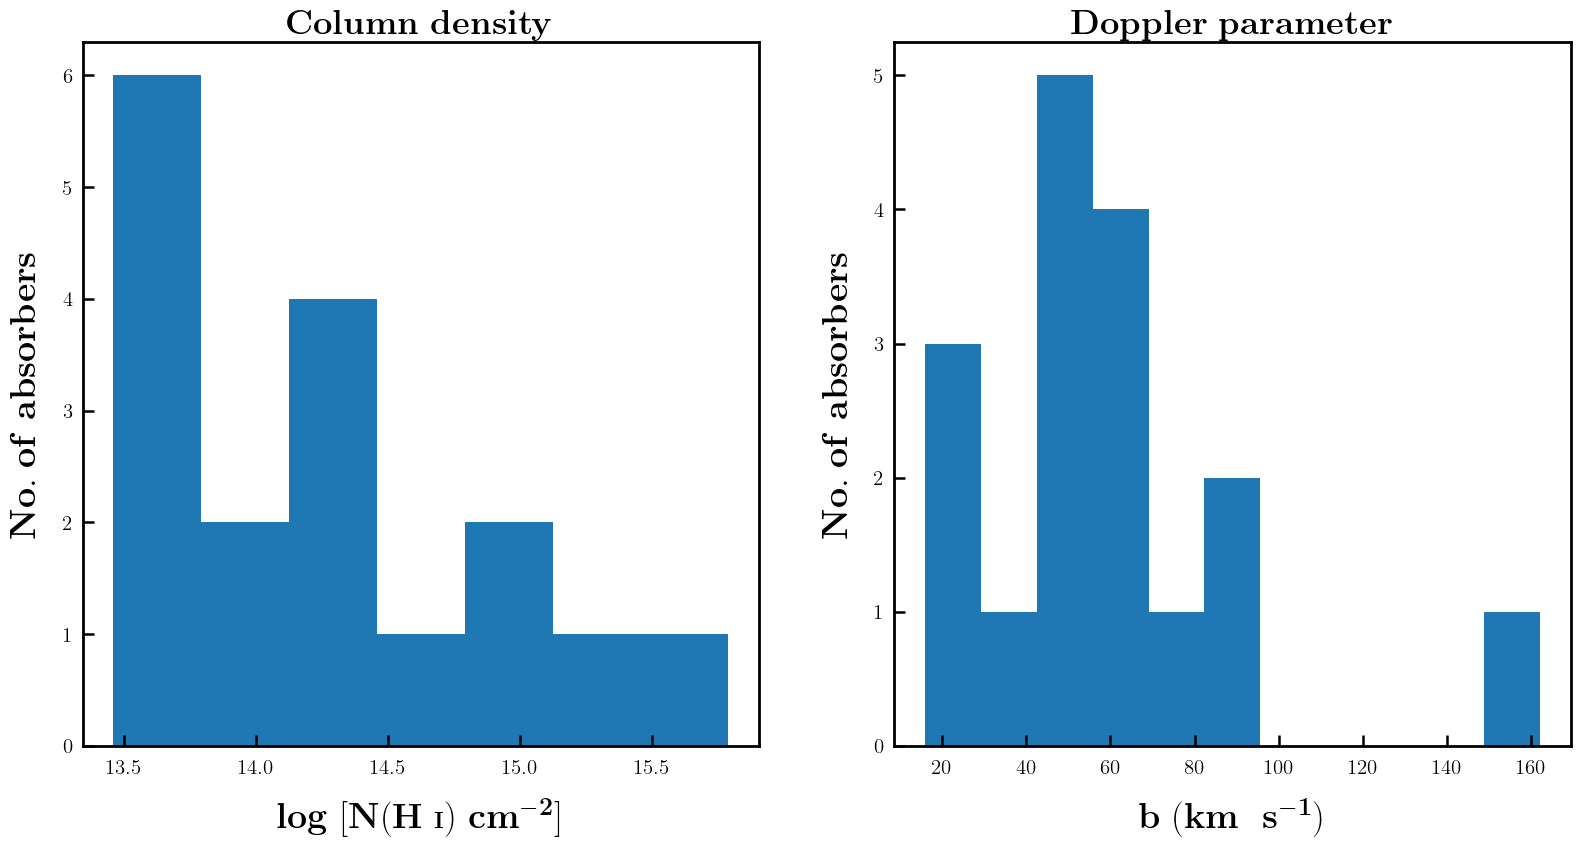
\includegraphics[width=0.9\linewidth]{Distribution_NH_b.png}
    \caption{Distribution of column density and doppler parameters of the Lyman lines in the 17 absorbers}
    \end{figure}
    
\begin{figure}[!b]
\centering
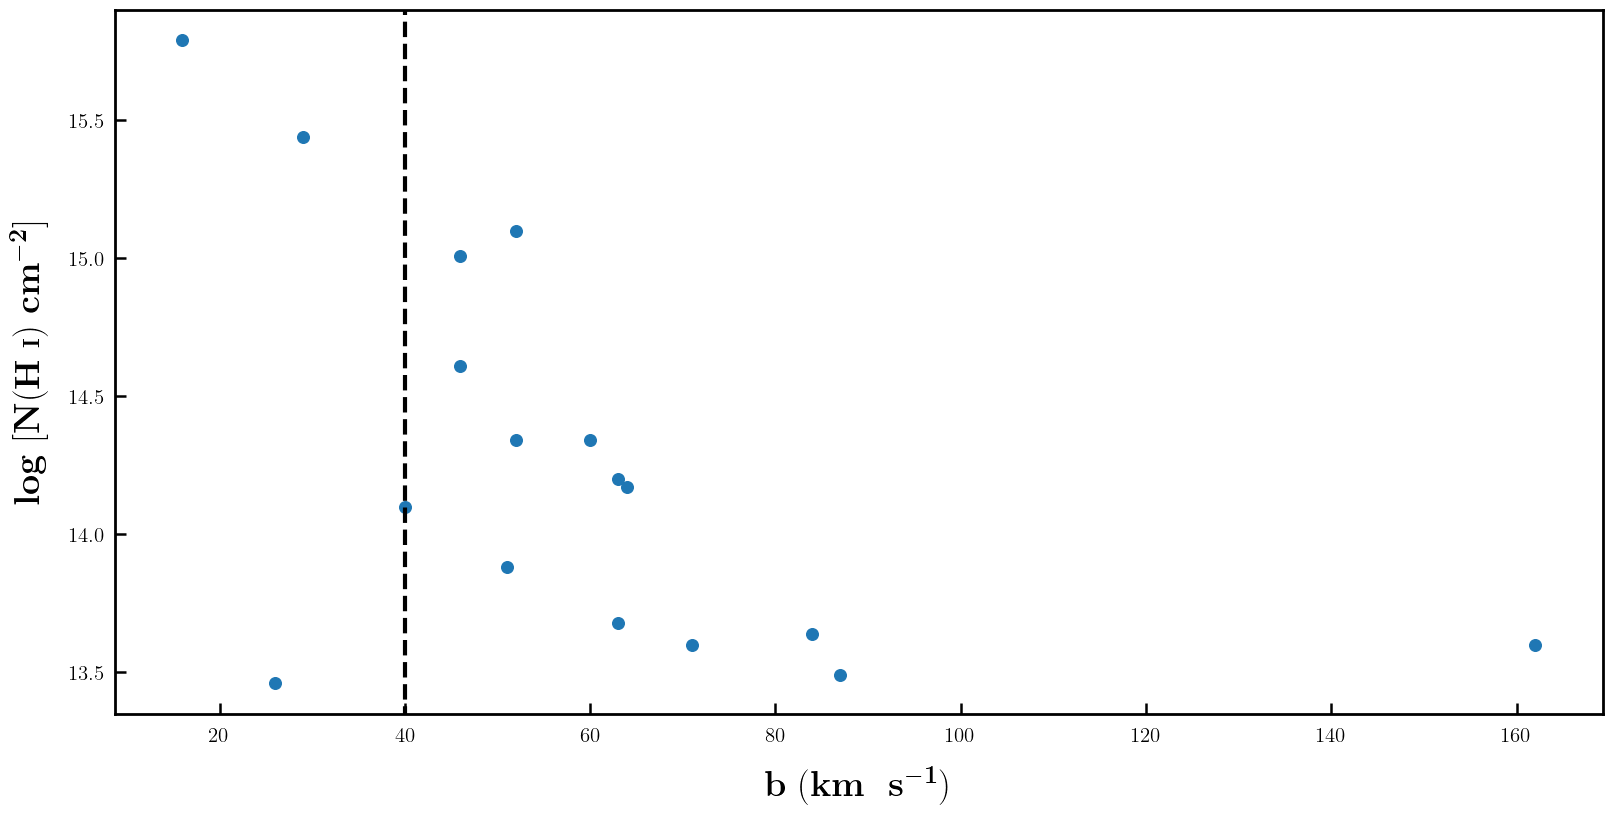
\includegraphics[width=0.9\linewidth]{NH_vs_b_1.png}
\caption{Column desnity v/s doppler parameter. Vertical black dashed line shows the doppler parameter of 40 km s$^{-1}$}
\end{figure}


\begin{figure}[!h]
    \centering
    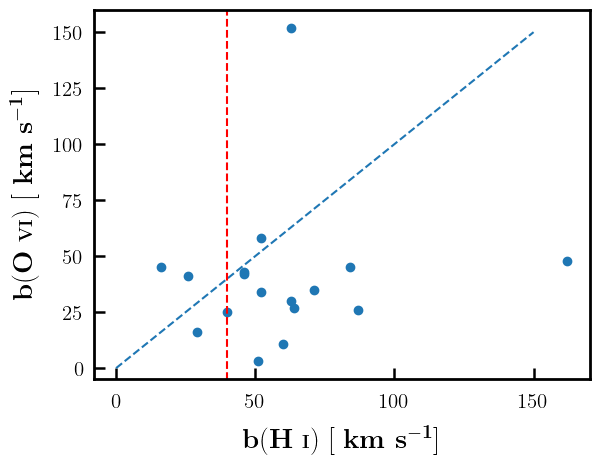
\includegraphics[width=\linewidth]{bHi_vs_BOvi.png}
    \caption{b(\ion{H}{i}) v/s b(\ion{O}{vi}). Vertical red dashed line shows the doppler parameter of 40 km s$^{-1}$. And blue dashed line shows the b(\ion{H}{i}) = b(\ion{O}{vi}) line}
\end{figure}


\end{document}
